\subsection{Example \#2 -- the roulette wheel}
Here, the outcome is binary -- we either win or lose. The probability of winning if we choose the red color, is $18/37$.
Let's simulate 40 bets at the roulette wheel, where, in each we put a dollar on red. Each bet is won with a Bernoulli distribution, $Ber(18/37)$ and we repeat it 40 times. Equivalently, we can look at it as a single binomial sample, with $n=40$ and $p=18/37$.

\begin{knitrout}
\definecolor{shadecolor}{rgb}{0.969, 0.969, 0.969}\color{fgcolor}\begin{kframe}
\begin{alltt}
\hlkwd{set.seed}\hlstd{(}\hlnum{75473}\hlstd{)}
\hlstd{n} \hlkwb{<-} \hlnum{40}
\hlstd{samp} \hlkwb{<-} \hlkwd{rbinom}\hlstd{(n,} \hlkwc{size}\hlstd{=}\hlnum{1}\hlstd{,} \hlkwc{prob}\hlstd{=}\hlnum{18}\hlopt{/}\hlnum{37}\hlstd{)}
\hlkwd{cat}\hlstd{(}\hlstr{"Mean="}\hlstd{,}\hlkwd{mean}\hlstd{(samp),} \hlstr{", SD="}\hlstd{,}\hlkwd{sd}\hlstd{(samp),}\hlstr{"\textbackslash{}n"}\hlstd{)}
\end{alltt}
\begin{verbatim}
## Mean= 0.575 , SD= 0.5006406
\end{verbatim}
\end{kframe}
\end{knitrout}

Notice that in those 40 bets, our probability of winning was 0.575 (greater than 0.5.) This seems great -- if we keep going we might get rich. However, let's see what happens to the sample mean as we increase $n$. 

\begin{knitrout}
\definecolor{shadecolor}{rgb}{0.969, 0.969, 0.969}\color{fgcolor}\begin{kframe}
\begin{alltt}
\hlkwd{set.seed}\hlstd{(}\hlnum{95473}\hlstd{)}
\hlstd{ns} \hlkwb{<-} \hlkwd{seq}\hlstd{(}\hlnum{10}\hlstd{,} \hlnum{2000}\hlstd{,} \hlkwc{by}\hlstd{=}\hlnum{10}\hlstd{)}
\hlstd{L} \hlkwb{<-} \hlkwd{length}\hlstd{(ns)}
\hlstd{allMeans} \hlkwb{<-} \hlkwd{rep}\hlstd{(}\hlnum{0}\hlstd{, L)}
\hlkwa{for} \hlstd{(i} \hlkwa{in} \hlnum{1}\hlopt{:}\hlstd{L) \{}
  \hlstd{samp} \hlkwb{<-} \hlkwd{rbinom}\hlstd{(ns[i],} \hlkwc{size}\hlstd{=}\hlnum{1}\hlstd{,} \hlkwc{prob}\hlstd{=}\hlnum{18}\hlopt{/}\hlnum{37}\hlstd{)}
  \hlstd{allMeans[i]} \hlkwb{<-} \hlkwd{mean}\hlstd{(samp)}
\hlstd{\}}
\hlkwd{plot}\hlstd{(ns, allMeans,} \hlkwc{pch}\hlstd{=}\hlnum{19}\hlstd{,} \hlkwc{cex}\hlstd{=}\hlnum{0.5}\hlstd{,} \hlkwc{col}\hlstd{=}\hlnum{3}\hlstd{,} \hlkwc{axes}\hlstd{=}\hlnum{FALSE}\hlstd{)}
\hlkwd{axis}\hlstd{(}\hlnum{1}\hlstd{);} \hlkwd{axis}\hlstd{(}\hlnum{2}\hlstd{)}
\hlkwd{abline}\hlstd{(}\hlkwc{h}\hlstd{=}\hlnum{18}\hlopt{/}\hlnum{37}\hlstd{,} \hlkwc{lwd}\hlstd{=}\hlnum{3}\hlstd{,}\hlkwc{col}\hlstd{=}\hlnum{2}\hlstd{)}
\end{alltt}
\end{kframe}\begin{figure}

{\centering 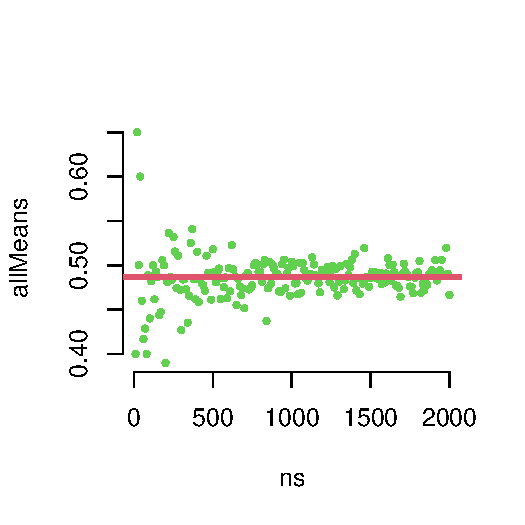
\includegraphics[width=\maxwidth]{figure/intro-lln1-2-1} 

}

\caption[The sample mean from n bets at the roulette wheel]{The sample mean from n bets at the roulette wheel.}\label{fig:intro-lln1-2}
\end{figure}

\end{knitrout}

As before, the sample mean gets closer to the true mean of the distribution, which is $p=18/37$, which is less than 0.5, so if we keep placing bets we will end up losing money. In fact, we can check how much we will lose if we bet \$1 each time, and do it 10,000 time

\begin{knitrout}
\definecolor{shadecolor}{rgb}{0.969, 0.969, 0.969}\color{fgcolor}\begin{kframe}
\begin{alltt}
\hlstd{n} \hlkwb{<-} \hlnum{10000}
\hlstd{roulette} \hlkwb{<-} \hlkwd{rbinom}\hlstd{(n,} \hlnum{1}\hlstd{,} \hlnum{18}\hlopt{/}\hlnum{37}\hlstd{)}
\hlkwd{cat}\hlstd{(}\hlstr{"Prob. win="}\hlstd{,} \hlkwd{mean}\hlstd{(roulette),}\hlstr{"\textbackslash{}n"}\hlstd{)}
\end{alltt}
\begin{verbatim}
## Prob. win= 0.4898
\end{verbatim}
\begin{alltt}
\hlkwd{cat}\hlstd{(}\hlstr{"Paid: $"}\hlstd{,} \hlkwd{prettyNum}\hlstd{(n,} \hlkwc{big.mark}\hlstd{=}\hlstr{","}\hlstd{),} \hlstr{". Won: "}\hlstd{,} \hlkwd{sum}\hlstd{(roulette),} \hlstr{"times."}\hlstd{,} \hlstr{"Total gain:"}\hlstd{,} \hlkwd{prettyNum}\hlstd{(}\hlnum{2}\hlopt{*}\hlkwd{sum}\hlstd{(roulette),} \hlkwc{big.mark} \hlstd{=} \hlstr{","}\hlstd{),} \hlstr{"dollars. Net gain/loss:"}\hlstd{,} \hlkwd{prettyNum}\hlstd{(}\hlnum{2}\hlopt{*}\hlkwd{sum}\hlstd{(roulette)}\hlopt{-}\hlstd{n,}\hlkwc{big.mark} \hlstd{=} \hlstr{","}\hlstd{),}\hlstr{"\textbackslash{}n"}\hlstd{)}
\end{alltt}
\begin{verbatim}
## Paid: $ 10,000 . Won:  4898 times. Total gain: 9,796 dollars. Net gain/loss: -204
\end{verbatim}
\end{kframe}
\end{knitrout}

To the casino it doesn't matter if one person bets \$1,000,000 or if 1,000 people each bets on \$1,000 -- in both cases the casino will win with probability 19/37.
